\section{应用时间序列部分}
\begin{center}
    Instructor: Dong Li
\end{center}

% Time series modelling usually concerns \textbf{forecasting}, i.e. predict future behaviour of a quantity based on history information. A direct method is modelling a time series object, with history and future are included in it. In this section several modelling/forecasting methods would be included.

\subsection{Time Series Data and Model}


\subsubsection{Time Series Data and Tasks}
    \textbf{Time Series} : a sequential r.v. indexed in time order.\index{Time Series}
    \begin{equation}
        \{Y_t\},\,t\in \mathcal{T}\quad \mathcal{T}\text{ is index set} 
    \end{equation}

    and actual data of time series, i.e. times series data is called a \textbf{Realization}  of time series, denoted\footnote{A note on $ T\subset \mathcal{T} $: actually $ T $ has to be discrete beacuse it is a sample of $ \mathcal{T} $. while $ \mathcal{T} $ is not necessarily defined as discrete.}
    \[
        \{y_t\},\,t\in  T\subset\mathcal{T}
    \]
    e.g. in forecasting task, $ T $ encodes history. In this chapter we usually focus on easier case of arithmetic progression $ T=\{1,2,\dots,N\} $, or at least numeric orderal sequence.

    Time Series Analysis (TSA)\index{TSA (Time Series Analysis)}: Analysis on time series data to extract meaningful statistics/other characteristics. Task of TSA includes:
    \begin{itemize}[topsep=2pt,itemsep=0pt]
        \item Describing and Explanaing the machanism of time series 
        \item Forecasting
        \item Guiding the intervention of Time Series
    \end{itemize}

    In this section several modelling/forecasting methods would be included.
    
    % Classification:
    % \begin{itemize}[topsep=2pt,itemsep=0pt]
    %     \item Standard: dimensionality:
    %     \begin{itemize}[topsep=2pt,itemsep=0pt]
    %         \item univariate
    %         \item multivariate
    %         \item high-dimensional: e.g. tensor
    %     \end{itemize}
    %     \item Standard: Regularity of sampling time
    %     \begin{itemize}[topsep=2pt,itemsep=0pt]
    %         \item regular TS
    %         \item irregular TS
    %     \end{itemize}
    %     \item Standard: Discrete/Continuous, including data discrete/continuous or time discrete/continuous. Most common: discrete time$ + $continuous data      
    % \end{itemize}

\subsubsection{Time Series Model}
    There are plenty of useful modelling methods:
    \begin{itemize}[topsep=2pt,itemsep=0pt]
        \item Regression Model: View $ y $ as function of $ t $, regression on some model $ y=f(t) $ with loss $ \mathcal{L} $. e.g. linear regression
        \begin{align*}
            y=\beta _0+\beta _1t+\varepsilon ,\quad \mathcal{L}=\sum_{t\in T}(y_t-\hat{y}_t)^2 
        \end{align*}
        
        Modelling strategy is similar to that introduced in linear regression, see \autoref{SecLinearRegressionAnalysis} 
        
        \item STL Method: Seasonal and Trend decomposition using Loess. A decomposition of time series into `TS = Trend + Season + Random', i.e.\index{STL Model (Seasonal and Trend Decomposition using Loess)}
        \begin{equation}
            Y_\tau=T_\tau+S_\tau+X_\tau 
        \end{equation}
    
        and we could model $ T_\tau $, $ S_{\tau} $, $ X_\tau $ separately. The focus is the modelling of random term $ X_t $, which we expect to be `stationarily random' through time. (Usually we model this part also by ARMA model)

        \item Exponential Smoothing Model: Use weighted average over history to predict future.

        \item ARIMA Model: The main focus of this chapter.
    \end{itemize}
    

    % where randomness lies in the (usually a zero mean stationary sequence) random term $ X_\tau $. After modelling non-random $ T_\tau  $, $ S_\tau  $, our target is to estimate the zero-mean stationary $ R_\tau \equiv X_\tau  $ based on history till $ t $ ($ \tau>t $).





\subsection{Stochastic Process and Statistics}
\subsubsection{Basic Knowledge of Stochastic Process}
    A stochastic process can be denoted:\index{Stochastic Process}
    \begin{equation}
        \{X_t:\,t\in \mathcal{T}\}:\, \Omega\times \mathcal{T}\to \mathcal{E}
    \end{equation}
    
\begin{point}
    Some important cases of stochastic process:
\end{point}

    
    \begin{itemize}[topsep=2pt,itemsep=0pt]
        \item i.i.d. sequence: $ \varepsilon _t\,\mathrm{i.i.d.}\sim \varepsilon   $        
        \item White Noise\index{WN (White Noise)}: uncorrelated for different subscript $ t $ in the sense of $ 2^\mathrm{nd}  $ moment, $ \varepsilon _t\sim \mathrm{WN}(\mu ,\sigma ^2)  $. where
        \begin{align*}
            \mathbb{E}\left( \varepsilon _t \right) =&\mu \\
            cov(\varepsilon _t,\varepsilon _s)=&\sigma ^2\delta _{t,s}
        \end{align*}

        Further we can append more constraints on $ \mathrm{WN}  $:
        \begin{itemize}[topsep=2pt,itemsep=0pt]
            \item[+] $ \{\varepsilon _t\} $ independent: independent white noise $ \varepsilon _t\sim \mathrm{IWN}(\mu ,\sigma ^2)  $ 
            \item[+] $ \mu =0 $: zero-mean white noise $ \varepsilon _t\sim \mathrm{WN}(0 ,\sigma ^2)  $
            \item[+] $ \mu =0 $, $ \sigma ^2=1 $: standard white noise $ \varepsilon _t\sim \mathrm{WN}(0,1)  $
            \item[+] $ \varepsilon \sim N(\mu ,\sigma ^2) $: normal white noise.
        \end{itemize}
        \item Martingale difference sequence (MDS)\index{MDS (Martingale Difference Sequence)}: zero expectation given history information: $ \varepsilon _t\sim \mathrm{MDS}  $, where
        \begin{align*}
            \mathbb{E}\left( |\varepsilon _t| \right) <&\infty\\
            \mathbb{E}\left( \varepsilon _t|\mathcal{F}_{t-1} \right) =&0
        \end{align*}

        where $ \mathcal{F}_\tau $ denotes the history until time $ \tau $:
        \begin{equation}
            \mathcal{F}_\tau\equiv \sigma \left(\varepsilon _s,\, s\leq \tau\right)\{\varepsilon _s,\varepsilon _{s-1},\varepsilon _{s-2},\ldots\} 
        \end{equation}
    \end{itemize}

    Relation: i.i.d. $ > $ MDS $ > $ WN $ > $ Stationary
    

{
\begin{figure}[H]
    \centering
    \tikzset{every picture/.style={line width=0.75pt}} %set default line width to 0.75pt        

    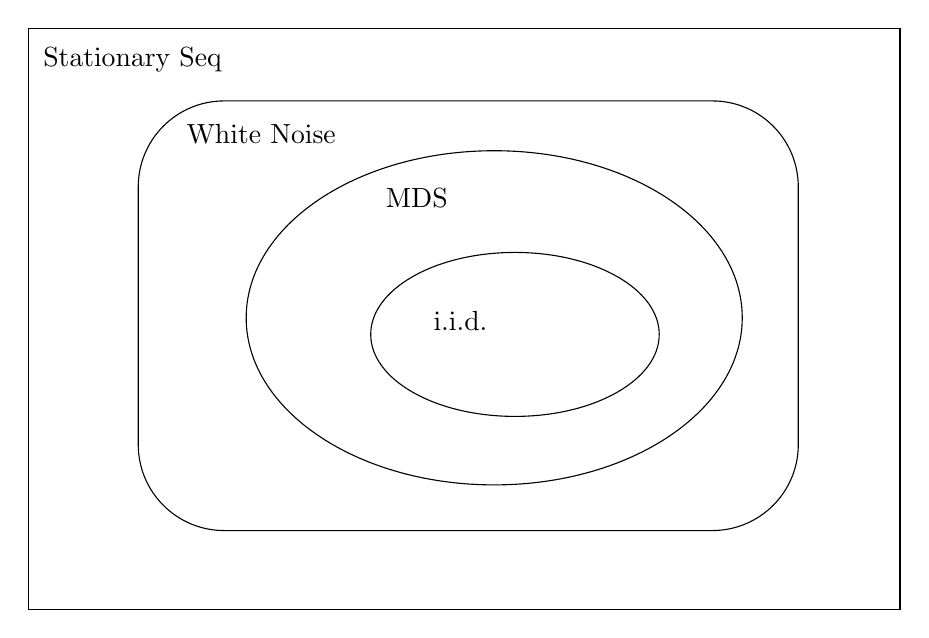
\begin{tikzpicture}[x=0.75pt,y=0.75pt,yscale=-1,xscale=1]
    %uncomment if require: \path (0,300); %set diagram left start at 0, and has height of 300
    
    %Shape: Rectangle [id:dp7367101782277172] 
    \draw   (115,13) -- (535.01,13) -- (535.01,293.02) -- (115,293.02) -- cycle ;
    %Rounded Rect [id:dp15861413740766106] 
    \draw   (168.01,89.42) .. controls (168.01,66.55) and (186.54,48.02) .. (209.41,48.02) -- (444.61,48.02) .. controls (467.47,48.02) and (486.01,66.55) .. (486.01,89.42) -- (486.01,213.62) .. controls (486.01,236.48) and (467.47,255.02) .. (444.61,255.02) -- (209.41,255.02) .. controls (186.54,255.02) and (168.01,236.48) .. (168.01,213.62) -- cycle ;
    %Flowchart: Connector [id:dp04508204736671462] 
    \draw   (220.01,152.52) .. controls (220.01,108.06) and (273.51,72.02) .. (339.51,72.02) .. controls (405.51,72.02) and (459.01,108.06) .. (459.01,152.52) .. controls (459.01,196.98) and (405.51,233.02) .. (339.51,233.02) .. controls (273.51,233.02) and (220.01,196.98) .. (220.01,152.52) -- cycle ;
    %Flowchart: Connector [id:dp3377595494528831] 
    \draw   (280.01,160.52) .. controls (280.01,138.7) and (311.13,121.02) .. (349.51,121.02) .. controls (387.89,121.02) and (419.01,138.7) .. (419.01,160.52) .. controls (419.01,182.33) and (387.89,200.02) .. (349.51,200.02) .. controls (311.13,200.02) and (280.01,182.33) .. (280.01,160.52) -- cycle ;
    
    
    % Text Node
    \draw (309,148) node [anchor=north west][inner sep=0.75pt]   [align=left] {i.i.d.};
    % Text Node
    \draw (286,89) node [anchor=north west][inner sep=0.75pt]   [align=left] {MDS};
    % Text Node
    \draw (190,58) node [anchor=north west][inner sep=0.75pt]   [align=left] {White Noise};
    % Text Node
    \draw (121,21) node [anchor=north west][inner sep=0.75pt]   [align=left] {Stationary Seq};
    
    
    \end{tikzpicture}
    \caption{Relation bet. Sequences}
\end{figure}
}


\begin{point}
    Measure of dependence within stochastic process
\end{point}

    Given a stochastic process $ \{X_t:\,t\in \mathcal{T}\} $

    \begin{itemize}[topsep=2pt,itemsep=0pt]
        \item Mean Function
        \begin{equation}
            \mu _t=\mathbb{E}\left( X_t \right)  
        \end{equation}        
        
        \item AutoCovariance Function (ACVF) and AutoCorrelation Function (ACF):\index{ACVF (Autocovariance)}\index{ACF (Autocorrelation)}
        \begin{align*}
            \text{ACVF: }\gamma _{t,s}\equiv &cov(X_t,X_s),& \mathcal{T}\times \mathcal{T}\to&\mathbb{R}\\
            \text{ACF: }\rho  _{t,s}\equiv &corr(X_t,X_s)=\dfrac{\gamma _{t,s}}{\sqrt[]{\gamma _{t,t}\gamma _{s,s}}},& \mathcal{T}\times \mathcal{T}\to& [-1,1]
        \end{align*}

        \item Stationarity: Stationarity is a measure that the `correlation structure of stochastic process looks the same' at any time $ t $, i.e. is stationary through time.
        \begin{itemize}[topsep=2pt,itemsep=0pt]
            \item Weakly Stationary (WS)\index{WS (Weakly Stationary)}: given $ \mathbb{E}\left( X_t^2 \right) < \infty $, has const mean and $ cov  $ independent of time
            \begin{align*}
                \mathbb{E}\left( X_t \right) =&\mu _t=\mu \\
                cov(X_t,X_t+k)=&\gamma _{t,t+k}=\gamma _k\independent t
            \end{align*}

            \item Strictly Stationary (SS)\index{SS (Strictly Stationary)}: joint distribution invariant through time. For any given $ \{t_1,t_2,\ldots,t_n\}\subset \mathcal{T} $
            \begin{equation}
                f_{X_{t_1},X_{t_2},\ldots,X_{t_n}}=f_{X_{t_1+h},X_{t_2+h},\ldots,X_{t_n+h}},\quad \forall h 
            \end{equation}
            
        \end{itemize}

        Some note on WS and SS:
        \begin{itemize}[topsep=2pt,itemsep=0pt]
            \item Generally speaking, WS and SS are not equivalant, WS $ \nLeftrightarrow $ SS (note that SS does not put constraint on $ \mathbb{E}\left( X_t^2 \right)  $)
            \item equivalent for gaussian stochastic process.
            \item ACF and ACVF of WS: 
            \begin{align*}
                \gamma _{t,t+k}=&\gamma _k=\gamma _{-k},\quad \forall t\in\mathcal{T}\\
                \rho _{t,t+k}=&\rho _k=\dfrac{\gamma _k}{\gamma _0},\quad\, \forall t\in\mathcal{T}
            \end{align*}

            Notation of ACVF matrix:
            \begin{equation}
                \Gamma _k=\{\gamma _{i-j}\}_{i,j=1}^k=\begin{bmatrix}
                    \gamma _0&\gamma _1&\gamma _2&\cdots&\gamma _{k-2}&\gamma _{k-1}\\
                    \gamma _1&\gamma _0&\gamma _1&\cdots&\gamma _{k-3}&\gamma _{k-2}\\
                    \gamma _2&\gamma _1&\gamma _0&\cdots&\gamma _{k-4}&\gamma _{k-3}\\
                    \vdots&\vdots&\vdots&\ddots&\vdots&\vdots\\
                    \gamma _{k-2}&\gamma _{k-3}&\gamma _{k-4}&\cdots&\gamma _0&\gamma _1\\
                    \gamma _{k-1}&\gamma _{k-2}&\gamma _{k-3}&\cdots&\gamma _1&\gamma _0
                \end{bmatrix}_{k\times k}
            \end{equation}

            $ \Gamma _k $ is semi-positive definite. 
            \begin{equation}
                \sum_{i=1}^k\sum_{j=1}^k\alpha _i\alpha_ j\gamma _{|t_i-t_j|}\geq 0,\quad \forall k,\{t_1,\ldots,t_k\} ,\vec{\alpha }
            \end{equation}
            
        \end{itemize}
        \item Partial Autocorrelation (PACF)\index{PACF (Partial Autocorrelation)}: correlation given information between two time points, orginal definition
        \begin{align}\label{EqaPartialAutoCorrelation}
            \phi _{11}=&\phi _1\\
            \phi _{kk}=&corr\big(X_t-L(X_t|X_{t+1},\ldots,X_{t+k-1}),X_{t+k}-L(X_{t+k}|X_{t+1},\ldots,X_{t+k-1})\big),\quad k\geq 2
        \end{align}

        where $ L(X_{\tau}|X_{t+1},\ldots,X_{t+k-1}) $ is the \textbf{Best Linear Estimation}  of linear model 
        \begin{align*}
             X_\tau = \beta _0+\beta _1X_{t+1}+\ldots+\beta _{k-1}X_{t+k-1}+\epsilon
        \end{align*}
        
           deduction:
        \begin{itemize}[topsep=2pt,itemsep=0pt]
            \item Best linear estimation $ \hat{X}_\tau \equiv L(X_\tau|X_{t+1},\ldots,X_{t+k-1}) $ satisfies 
            \begin{equation}
                \{\beta _0,\beta \}=\mathop{\arg\min}\limits_{\beta _0,\beta }  \mathbb{E}\left( \hat{X}_\tau-\beta _0-\sum_{j=1}^{k-1}\beta _jX_{t+j} \right)  ^2
            \end{equation}

            solution: denote $ X=(X_{t+1},\ldots,X_{t+k-1}) $, $ \beta =(\beta _1,\ldots,\beta _{k-1}) $
            \begin{align*}
                \hat{\beta }=&\Sigma ^{-1}_X\Sigma _{X,X_{\tau}}\\
                \hat{\beta }_0=&\mathbb{E}\left( X_{\tau} \right) -\mathbb{E}\left( X \right)' \hat{\beta }
            \end{align*}
            i.e.
            \begin{equation}\label{EqaBestLinearEstimationOfTS}
                L(X_\tau|X_{t+1},\ldots,X_{t+k-1}) =\mathbb{E}\left( X_{\tau} \right) + \Sigma _{X_\tau,X}\Sigma _X^{-1}(X-\mathbb{E}\left( X \right) )
            \end{equation}

            Simplified case for zero-mean Weakly Stationary $ \mathbb{E}(X_t)=\mu  $; $ \gamma _k $, $ \Gamma _k $
            \begin{align}\label{EqaBestLinearEstimationOfWSTS}
                L(X_{t+k}|X_{t+1},\ldots,X_{t+k-1}) =&\mathbb{E}\big( X_{t+k} \big) + \Sigma _{X_{t+k},X}\Sigma _X^{-1}(X-\mathbb{E}\left( X \right) )\\
                =&\gamma _{k-1}'\Gamma _{k-1}^{-1}X_{t+k-1:t+1}
            \end{align}
                
            
        \end{itemize}

        % then we could get 
        % \begin{align*}
        %     \phi _{kk}=&corr\left(X_t-L(X_t|X_{t+1},\ldots,X_{t+k-1}),X_{t+k}-L(X_{t+k}|X_{t+1},\ldots,X_{t+k-1})\right),\quad k\geq 2\\
        %     =&
        % \end{align*}

    
        Calculation formula for zero-mean Weakly Stationary:
        \begin{itemize}[topsep=2pt,itemsep=0pt]
            \item using determinant form
            \begin{align*}
            \phi _{11}=&\rho _1\\
            \phi _{kk}=&\dfrac{\begin{vmatrix}
                1&\rho _1&\rho _2&\cdots&\rho _{k-2}&{\color{red}\rho _1}\\
                \rho _1&1&\rho _1&\cdots&\rho _{k-3}&{\color{red}\rho _2}\\
                \vdots&\vdots&\vdots&\ddots&\vdots&{\color{red}\vdots}\\
                \rho _{k-1}&\rho _{k-2}&\rho _{k-3}&\cdots&\rho _1&{\color{red}\rho _k}
            \end{vmatrix}_{k\times k}}{\begin{vmatrix}
                1&\rho _1&\rho _2&\cdots&\rho _{k-2}&{\color{blue}\rho _{k-1}}\\
                \rho _1&1&\rho _1&\cdots&\rho _{k-3}&{\color{blue}\rho _{k-2}}\\
                \vdots&\vdots&\vdots&\ddots&\vdots&{\color{blue}\vdots}\\
                \rho _{k-1}&\rho _{k-2}&\rho _{k-3}&\cdots&\rho _1&{\color{blue}1}
            \end{vmatrix}_{k\times k}}
        \end{align*}
            
        \item Levinson-Durbin's recursive formula\index{Levinson-Durbin's Recursive Formula}
        \begin{align}\label{EqaLevinsonDurbin}
            \phi _{11}=&\rho _1\\
            \phi _{k+1,k+1}=&\dfrac{\rho _{k+1}-\sum_{j=1}^k\phi _{k,j}\rho _{k+1-j}}{1-\sum_{j=1}^k\phi _{k,j}\rho _j},\quad k\geq 1\\
            \phi _{k+1,j}=&\phi _{k,j}-\phi _{k+1,k+1}\phi _{k,k+1-j},\quad j=1,2,\ldots,k
        \end{align}
        
        where $ \phi _{k+1,j} $ here is a formal notation for recursion. But we will see its meaning in AR$ (p) $ model (\autoref{EqaLevinsonDurbinInARp})
        
        
    \end{itemize}
        
            
    

        \item Wold Decomposition\index{Wold Decomposition}: zero-mean weakly stationary time series can be decomposed as :
        \begin{equation}
            X_t=\sum_{j=-\infty}^\infty \phi _j\varepsilon _{t-j}+V_t 
        \end{equation}
        where
        \begin{align*}
            \phi _0=&1\\
            \varepsilon _t\sim &\mathrm{WN}(0,\sigma ^2) 
        \end{align*}


        \item Spectrum of zero-mean weak stationary time series $ \{X_t\} $:
        \begin{equation}
            X_t=\int _\lambda \xi (\lambda )e^{i\lambda t} \,\mathrm{d}\lambda 
        \end{equation}

        We can use this form to construct ACF, ACVF, etc.
        \begin{itemize}[topsep=2pt,itemsep=0pt]
            \item ACVF:
            \begin{align*}
                \gamma _k=&cov(X_t,X_{t+k})\\
                =&\mathbb{E}\left( X_t^*X_{t+k} \right)\\
                =&\int _{t}\int _{\lambda _1}\int _{\lambda _2} \xi ^*(\lambda _1)\xi  \,\mathrm{d}\lambda _2 e^{i(\lambda _2-\lambda _1)t+i\lambda _2k} f(t) \,\mathrm{d}\lambda _1 \,\mathrm{d}t \\
                =&\int _{\lambda _1}\int _{\lambda _2} \xi ^*(\lambda _1)\xi  \,\mathrm{d}\lambda _2  \,\mathrm{d}\lambda _1 \\
                =&\int _{\lambda _2}e^{-\lambda _2k} {\color{blue} \int _t\int _{\lambda_1} \xi ^*(\lambda _1)\xi  \,\mathrm{d}\lambda _2 e^{i(\lambda _2-\lambda _1)t} f(t) \,\mathrm{d}\lambda _1 \,\mathrm{d}t }  \,\mathrm{d}\lambda _2\\
                \equiv&\int _{\lambda } e^{-\lambda k}{\color{blue}\nu (\lambda )}  \,\mathrm{d}\lambda 
            \end{align*}
            here function $ F(\lambda )=\int \nu (\lambda ) \,\mathrm{d}\lambda  $ is the \textbf{spectrum} of $ \gamma _k $ 

            For $ k=0,1,2,\ldots $:
            \begin{equation}
                \gamma _k=\int _{-\pi}^\pi \nu (\lambda )e^{i\lambda k} \,\mathrm{d}\lambda  
            \end{equation}
            
            and also use inverse fourier transform: for weak stationary TS $ X_t=\sum_{j=-\infty}^\infty \phi _j\varepsilon _{t-j} $, $ \varepsilon _t\sim \mathrm{WN}(0,\sigma ^2)  $
            \begin{equation}
                \nu (\lambda )= \dfrac{\sigma ^2}{2\pi}\left\vert \sum_{j=-\infty}^\infty \phi _je^{i\lambda j} \right\vert ^2
            \end{equation}
            
            
            
        \end{itemize}
        
            

        
        
        
    \end{itemize}

\begin{point}
    Statistics
\end{point}

    To estimate the above $ \mu _t=\mu $, $ \gamma _k $, $ \rho _k $, $ \phi _{kk} $ given a realization of $ \{X_t\} $, say we have $ \{x_t\}_{t=1}^n $, we can construct:
    \begin{itemize}[topsep=2pt,itemsep=0pt]
        \item Sample mean $ \mu  $:
        \begin{equation}
            \hat{\mu }=\hat{x}_n=\dfrac{1}{n}\sum_{t=1}^nx_t 
        \end{equation}

        $ \hat{\mu } $ is the unbiased, consistent estimator, with
        \[
            \sqrt[]{n}(\hat{\mu }-\mu )\xrightarrow[]{\mathscr{L}} N(0,\sigma ^2) 
        \]
        
        an estimator using spectrum:
        \begin{align}
            &\sqrt[]{n}(\hat{\mu }-\mu )\xrightarrow[]{\mathscr{L}} N(0,2\pi \nu (0))\\
            &2\pi \nu (0)=\gamma _0+2\sum_{j=1}^\infty \gamma _j=\sum_{j=-\infty}^\infty \gamma _j 
        \end{align}
        
        \item ACVF $ \gamma _k $:
        \begin{align*}
            \hat{\gamma }_k=&\dfrac{1}{n}\sum_{t=1}^{n-k}(x_t-\hat{\mu })(x_{t+k}-\hat{\mu }) \\
            \hat{\hat{\gamma }}_k=&\dfrac{1}{n-k}\sum_{t=1}^{n-k}(x_t-\hat{\mu })(x_{t+k}-\hat{\mu }) 
        \end{align*}

        Note for actual usage:
        \begin{itemize}[topsep=2pt,itemsep=0pt]
            \item We usually avoid estimation for $ k\to n $ due to large error when $ n-k $ is small
            \item In most cases we use $ \hat{\gamma }_k $ rather than $ \hat{\hat{\gamma }}_k $, for two reasons:
            \begin{itemize}[topsep=2pt,itemsep=0pt]
                \item We often estimate $ \gamma _k $ for small $ k $, which means $ \hat{\gamma }_k\approx \hat{\hat{\gamma }}_k $
                \item $ \hat{\gamma }_k $ could guarantee the semi-positive-definition of $ \hat{\Gamma }_k $:
                \[
                     \hat{\Gamma }_k=\{\hat{\gamma }_{i-j}\}_{i,j=1}^k
                \]
            \end{itemize}
            
            asymptotic distribution: denote i.i.d. standard normal time series $ W_t\sim \mathrm{i.i.d.} \,N(0,1)  $
            \begin{align}
                &\sqrt[]{n}(\hat{\gamma }_0-\gamma _0,\hat{\gamma }_1-\gamma _1,\ldots,\hat{\gamma }_h-\gamma _h)\xrightarrow[]{\mathscr{L}} (\xi _0,\xi _1,\ldots,\xi _h)\\
                &\xi _j=(\dfrac{\sqrt[]{\mathbb{E}\left( \varepsilon ^4 \right) -\sigma ^4}}{\sigma ^2}\gamma _j)W_0+\sum_{t=1}^\infty (\gamma _{t+j}+\gamma _{t-j})W_t,\quad j\geq 0
            \end{align}
                
        \end{itemize}
        
            
        \item ACF $ \rho _k $:
        \begin{align*}
            \hat{\rho }_k=\dfrac{\hat{\gamma }_k}{\hat{\gamma }_0}=\dfrac{\sum_{t=1}^{n-k}(x_t-\hat{\mu })(x_{t+k}-\hat{\mu })}{\sum_{t=1}^{n-k}(x_t-\hat{\mu })^2}
        \end{align*}

        asymptotic distribution: denote i.i.d. standard normal time series $ W_t\sim \mathrm{i.i.d.} \,N(0,1)  $
        \begin{align}\label{EqaEstimationDistributionOfACF}
            &\sqrt[]{n}(\hat{\gamma }_0-\gamma _0,\hat{\gamma }_1-\gamma _1,\ldots,\hat{\gamma }_h-\gamma _h)\xrightarrow[]{\mathscr{L}} (R _0,R _1,\ldots,R _h)\\
            &R _j=\sum_{t=1}^\infty(\phi _{t+j}\rho _{t-j}-2\rho _t\rho _j)W(t),\quad j\geq 1
        \end{align}
        \item PACF $ \phi _{kk} $: take $ \hat{\rho }_k $ in the calculation equation of $ \phi _{kk} $.
    \end{itemize}
    
        


\subsection{ARMA Model}
    Two of the basic modeling methods for time series: Auto-Regression (AR) and Moving-Average (MA)
    
\subsubsection{Backshift Operator and Difference Equation}

\begin{point}
    Backshift Operator $ \mathscr{B}  $
\end{point}

    For clearer notation of ARMA and induce the solution, we first introduce backshift operator $ \mathscr{B}  $ of time series: given time series $ \{X_t\} $\footnote{Backshift operator could be used to construct difference operator $ \Delta =(1-\mathscr{B} ) $, e.g.
    \begin{align*}
        \Delta X_t&=(1-\mathscr{B} )X_t=X_t-X_{t-1}\\
        \Delta ^2X_t=&(1-\mathscr{B} )^2X_t=X_t-2X_{t-1}+X_{t-2}\\
        \ldots&
    \end{align*}
    
    or seasonal difference operator $ \Delta _k=(1-\mathscr{B} ^k) $, e.g.
    \begin{equation}
        \Delta _4X_t=(1-\mathscr{B} ^4)=X_t-X_{t-4} 
    \end{equation}
    
    }
    \begin{equation}
         \mathscr{B} X_t=X_{t-1},\quad \forall t
    \end{equation}
    
    further it can be used as variable of function by Laurant function series expansion:
    \begin{align*}
        \psi (z)=&\sum_{j=-\infty}^\infty \psi _{j}z^j\\
        \psi (\mathscr{B} )=&\sum_{j=-\infty}^\infty \psi _{j}\mathscr{B}^j \\
        \psi (\mathscr{B} )X_t=&\sum_{j=-\infty}^\infty \psi _{j}\mathscr{B}^jX_t=\sum_{j=-\infty}^\infty \psi _{j}X_{t-j}
    \end{align*} 

    for time series $ \{X_t\} $, $ \{Y_t\} $. r.v. $ U,V,W $:
    \begin{equation}
        \phi (\mathscr{B} )(UX_t+VY_t+W)=U\psi (\mathscr{B} )X_t+V\psi (\mathscr{B} )Y_t+W\psi (1) 
    \end{equation}

\begin{point}
    Difference Equation
\end{point}

    $ p^\mathrm{th}  $ order ordinary difference equation:
    \begin{equation}
        X_t-\left[a_1X_{t-1}+a_2X_{t-2}+\ldots+a_pX_{t-p}\right]=0 
    \end{equation}
    can be solved using backshift operator: define characteristic equation which would have $ p $ roots $ \zeta _j $
    \begin{align*}
        A(z)=&1-\left[a_1z+a_2z^2+\ldots+a_pz^p\right]\\
        =&1-\sum_{j=1}^pa_jz^j\\
        =&\prod_{j=1}^p(1-\zeta _jz)\\
        A(\mathscr{B} )=&1-\sum_{j=1}^pa_j\mathscr{B} ^j\\
        =&\prod_{j=1}^p(1-\zeta _j\mathscr{B} )
    \end{align*}
    
    similar to ODE, we can construct general solution from $ \zeta _j $, and particular solution.\footnote{Cases for multiple root see \url{https://www.math.pku.edu.cn/teachers/lidf/course/atsa/atsanotes/html/_atsanotes/atsa-lagdiff.html}}

\subsubsection{AR Model}
\index{AR Model (Auto-Regression Model)}
    Auto-Regression model (of order $ p $) contains ($ p^\mathrm{th} $ order) backshift on $ X_t $:
    \begin{equation}
        X_t=\phi _1X_{t-1}+\phi _2X_{t-2}+\ldots+\phi _pX_{t-p}+\varepsilon _t,\quad \varepsilon _t\sim \mathrm{WN}(\mu_\varepsilon  ,\sigma ^2)  
    \end{equation}
    or expressed in backshift operator with $ \phi (z)=1-\sum_{j=1}^p\phi _jz^j $, where the root of $ \phi (z)=0 $ denoted $ \alpha _j $
    \begin{align*}
        &\phi (\mathscr{B} )X_t=\varepsilon _t,\quad\varepsilon _t\sim \mathrm{WN}(\mu_\varepsilon  ,\sigma ^2)   \\
        &\phi (z)=1-\sum_{j=1}^p\phi _jz^j=\prod_{j=1}^p(1-\alpha _jz)
    \end{align*}

\begin{point}
    Properties and Solution: (here we consider stationary case $ \mu_\varepsilon  =0 $)
\end{point}

    \begin{itemize}[topsep=2pt,itemsep=0pt]
        \item (Weak) Stationarity condition: 
        \begin{equation}
            |\alpha _j| > 1,\,\forall j
        \end{equation}
        
        \item Solution of $ X_t $: using the expansion of $ \phi ^{-1} $
        \begin{align*}
            \phi (z)=&1-\sum_{j=1}^p\phi _jz^j\\
            \phi ^{-1}(z)=&\sum_{j=0}^\infty \psi _{j}z^j,\quad \psi _0=1
        \end{align*}

        naturally expressed in the form of Wold Decomposition:
        \begin{align*}
            \phi (\mathscr{B} )X_t=\varepsilon _t\Rightarrow & X_t=\phi ^{-1}(\mathscr{B} )\varepsilon _t=\sum_{j=0}^\infty \psi _j\varepsilon _{t-j},\quad \psi _0=1
        \end{align*}

        \item ACF and ACVF:
        \begin{align*}
            \gamma _k=&\sigma ^2\sum_{j=0}^\infty \psi _j\psi _{j+k}\\
            \rho _k=&\dfrac{\sum_{j=0}^\infty\psi _j\psi _{j+k}}{\sum_{j=0}^\infty\psi _j^2}
        \end{align*}
        \item Spectrum density $ \nu (\lambda ) $:
        \begin{align*}
            \nu  (\lambda )=&\dfrac{\sigma ^2}{2\pi}\left\vert \sum_{j=0}^\infty \psi _je^{i\lambda j} \right\vert^2\\
            =& \dfrac{\sigma ^2}{2\pi}\left\vert\phi ^{-1}(e^{i\lambda })\right\vert^2
        \end{align*}
        \item Yule-Walker Equation\index{Y-W Equation (Yule-Walker Equation)}: we have
        \begin{align*}
            \mathbb{E}\left( X_tX_{t-k} \right) =&\phi _1\mathbb{E}\left( X_{t-1}X_{t-k} \right) +\ldots+\phi _p\mathbb{E}\left( X_{t-p}X_{t-k} \right) +\mathbb{E}\left( \varepsilon _tX_{t-k} \right)  ,\quad \forall k=1,2,\ldots,p\\
            \Rightarrow \gamma _k=&\phi _1\gamma_{k-1}+\ldots+\phi _p\gamma _{k-p}, \quad \forall k=1,2,\ldots,p
        \end{align*}

        and for $ k=0 $:
        \begin{align*}
            \gamma _0=\phi _1\gamma _1+\ldots+\phi _p\gamma _p+\sigma ^2
        \end{align*}



        write in matrix form to get Yule-Walker Equation:
        
        \begin{align*}
            \begin{bmatrix}
                \gamma _1\\\gamma _2\\ \vdots\\\gamma _p
            \end{bmatrix} =&
            \begin{bmatrix}
                \gamma _0&\gamma _1&\cdots&\gamma _{p-1}\\
                \gamma _1&\gamma _0&\cdots&\gamma _{p-2}\\
                \vdots&\vdots&\ddots&\vdots\\
                \gamma _{p-1}&\gamma _{p-2}&\cdots&\gamma _0
            \end{bmatrix}
            \begin{bmatrix}
                \phi _1\\\phi _2\\ \vdots \\\phi _p
            \end{bmatrix}\\
            \sigma ^2 =& \gamma _0-\phi _1\gamma _1-\ldots-\phi _p\gamma _p
        \end{align*}
        
        or in dense matrix form (1):
        \begin{align*}
            \gamma =&\Gamma \phi \\
            \sigma ^2=&\gamma _0-\phi '\gamma 
        \end{align*}

        dense form (2):
        \begin{equation}
            \begin{bmatrix}
                -\sigma ^2\\ 0\\ 0 \\ \vdots \\0
            \end{bmatrix} =
            \begin{bmatrix}
                \gamma _0&\gamma _1&\gamma _2&\cdots &\gamma _p\\
                \gamma _1&\gamma _0&\gamma _1&\cdots&\gamma _{p-1}\\
                \gamma _2&\gamma _1&\gamma _0&\cdots&\gamma _{p-2}\\
                \vdots&\vdots&\vdots&\ddots&\vdots\\
                \gamma _p&\gamma _{p-1}&\gamma _{p-2}&\cdots&\gamma _0
            \end{bmatrix}
            \begin{bmatrix}
                -1\\\phi _1\\\phi _2\\ \vdots \\\phi _p
            \end{bmatrix}
        \end{equation}

        \item PACF: the coefficient of AR$ (p) $ has straight relation with $ \phi _{k,j} $: for all given $ k\geq p $
        \begin{align*}
            (\phi _1,\ldots,\phi _p,0,\ldots,0)=(\phi _{k,1},\ldots,\phi _{k,p},\phi _{k,p+1},\ldots,\phi _{k,k})
        \end{align*}

        (Note that $ \phi _{p,j}=\phi _{p+1,j}=\phi _{p+2,j}=\ldots $ using Levinson-Durbin' recursion \autoref{EqaLevinsonDurbin}).       
        
       
    \end{itemize}
    
\begin{point}
    Estimation: Key focus is the estimation of $ \phi _i,\,i=1,2,\ldots,p $ and $ \sigma ^2 $ (assume a TS of $ \mu _\varepsilon =0 $)
\end{point}

    Y-W Estimation and OLS Estimation are moment methods, asymptotically the same. MLE Estimation is usually more precise, but hard to calculate.

    \begin{itemize}[topsep=2pt,itemsep=0pt]
        \item Yule-Walker Estimation: use $ \gamma =\Gamma \phi  $. First estimate $ \hat{\gamma } $, as well as $ \hat{\Gamma } $, and get estimation for $ \phi ,\sigma ^2 $
        \begin{align*}
            \hat{\phi }=& \hat{\Gamma }^{-1}\hat{\gamma }\\
            \hat{\sigma }^2=&\hat{\gamma }_0-\hat{\gamma }'\hat{\Gamma }^{-1}\hat{\gamma }
        \end{align*}

        Asymptotic distribution:
        \begin{equation}
            \sqrt{n}(\hat{\phi }-\phi )\xrightarrow[]{\mathscr{L}} N_p(0,\sigma ^2\Gamma ^{-1}) 
        \end{equation}
        

        \item Levinson-Durbin's recursion for Yule-Walker Estimation: since PACF are the same as coefficients $ \phi _{k,j}=\phi _j $, we can use Durbin's recursion to avoid calculation of $ \hat{\Gamma }^{-1} $
        \begin{align}\label{EqaLevinsonDurbinInARp}
            \hat{\phi} _{11}=&\hat{\rho} _1\\
            \hat{\phi} _{k+1,k+1}=&\dfrac{\hat{\rho} _{k+1}-\sum_{j=1}^k\hat{\phi} _{k,j}\hat{\rho} _{k+1-j}}{1-\sum_{j=1}^k\hat{\phi} _{k,j}\hat{\rho} _j},\quad k\geq 1\\
            \hat{\phi} _{k+1,j}=&\hat{\phi} _{k,j}-\hat{\phi} _{k+1,k+1}\hat{\phi} _{k,k+1-j},\quad j=1,2,\ldots,k\\
            \hat{\sigma} _0^2=&\hat{\gamma }_0\\
            \hat{\sigma}_k^2 =& \hat{\sigma}_{k-1}^2 (1 - \hat{\phi}_{k,k}^2)
        \end{align}

        estimator:
        \begin{equation}
            \hat{\phi }_j=\hat{\phi }_{p,j} 
        \end{equation}
        
        



        \item OLS Estimation: using the linear combination form of AR model:
        \begin{equation}
            \hat{\phi }=\mathop{\arg\min}\limits_{\phi } \sum_{t=p+1}^n \left[ x_t-\sum_{j=1}^p \phi _jx_{t-j} \right]^2
        \end{equation}
        
        the solution is in the form of OLS estimator $ (X'X)^{-1}XY $, with $ X,Y $ properly defined
        
        \item MLE Estimation: under normal assumption
        \begin{equation}
            \phi (\mathscr{B} )X_t=\varepsilon _t,\quad \varepsilon _t\sim N(0,\sigma ^2) 
        \end{equation}

        Likelihood: define $ \theta =\{\phi _1,\ldots,\phi _p,\sigma ^2\} $
        \begin{align*}
            L(\theta ; x_1,\ldots ,x_n)=&f(x_1,\ldots,x_p|\theta )\prod_{t=p+1}^nf(x_t|x_{t-1},\ldots,x_{1};\theta )\\
            \approx \propto &\prod_{t=p+1}^nf(x_t|x_{t-1},\ldots,x_{1};\theta )\\
            =&\prod_{t=p+1}^n \dfrac{1}{\sqrt[]{2\pi \sigma ^2}}\exp\left\{ -\dfrac{1}{2\sigma ^2}(x_t-\sum_{j=1}^p \phi _jx_{t-j})^2 \right\}\\
            =&(2\pi\sigma ^2)^{-(n-p)/2}\exp\left\{ -\dfrac{1}{2\sigma ^2}\sum_{t=p+1}^n (x_t-\sum_{j=1}^p \phi _jx_{t-j})^2\right\}
        \end{align*}
        
        \item Estimation to spectrum density:
        \begin{equation}
            \hat{\nu }(\lambda )=\dfrac{\hat{\sigma }^2}{2\pi}\left\vert 1-\sum_{j=1}^{\hat{p}}\hat{\phi }_je^{i\lambda j} \right\vert^{-2} 
        \end{equation}
        
    \end{itemize}
    
        


\subsubsection{MA Model}
\index{MA Model (Moving-Average Model)}

    Moving-Average model (of order$ q $) contains ($ q^\mathrm{th}  $ order) backshift on $ \varepsilon _t $:
    \begin{equation}
        X_t=\varepsilon _t+\theta _1\varepsilon _{t-1}+\ldots +\theta _q\varepsilon _{t-q},\quad \varepsilon _t\sim \mathrm{WN}(\mu_\varepsilon  ,\sigma ^2) 
    \end{equation}

    or expressed in backshift operator with $ \theta (z)=1+\sum_{j=1}^q\theta _jz^j $, where the root of $ \theta (z) =0$ denoted $ \kappa _j $
    \begin{align}
        X_t=&\theta (\mathscr{B} )\varepsilon _t,\quad \varepsilon _t\sim \mathrm{WN}(\mu _\varepsilon ,\sigma ^2)\\
        \theta (z)=&1+\sum_{j=1}^q\theta _jz^j=\prod_{j=1}^q(1-\kappa _jz)\\
        =&\sum_{j=0}^q\theta _jz^j,\quad \theta _j=1
    \end{align}

    here we could note that AR$ (p) $ model has solution in the form of MA$ (\infty) $:
    \begin{equation}
        \mathrm{AR}(p):X_t=\sum_{j=0}^\infty \psi _j\varepsilon _{t-j},\quad \psi _0=1  
    \end{equation}
    
    
    
\begin{point}
    Properties and Solution: (here we consider stationary case $ \mu _\varepsilon =0 $)
\end{point}

\begin{itemize}[topsep=2pt,itemsep=0pt]
    \item Invertibility: if and only if 
    \begin{equation}
        |\kappa _j|>1,\,\forall j
    \end{equation}
    
    
    \item ACF and ACVF:
    \begin{align}
        \gamma _k=&\begin{cases}
            \sigma ^2\sum_{j=0}^{q-k}\theta _j\theta _{j+k},&0\leq k\leq q\\
            0,&k>q
        \end{cases}\\
        \rho _k=&\begin{cases}
            \dfrac{\sum_{j=0}^{q-k}\theta _j\theta _{j+k}}{\sum_{j=0}^q \theta _j^2 },&0\leq k\leq q\\
            0,&k>q
        \end{cases}
    \end{align}

    \item Solution: $ \hat{\theta }_j $ could solved from $ \{\gamma _k\} $
\end{itemize}  


    

\subsubsection{ARMA Model}
    Auto-Regerssion-Moving-Average model\index{ARMA Model} ARMA$ (p,q) $ in the form of 
    \begin{align}
        &\phi (\mathscr{B} )X_t=\theta (\mathscr{B} )\varepsilon _t\\
        &\phi (z)=1-\sum_{j=1}^p \phi _jz^j=\prod_{j=1}^p(1-\alpha _jz)\\
        &\theta (z)=1+\sum_{j=1}^q\theta _jz^j=\prod_{j=1}^q(1-\kappa _jz)
    \end{align}
    
    
    \begin{point}
        Properties and Solution: (here we consider stationary case $ \mu _\varepsilon =0 $)
    \end{point}

    \begin{itemize}[topsep=2pt,itemsep=0pt]
        \item Solution:
        \begin{equation}
            X_t=\phi ^{-1}(\mathscr{B} )\theta (\mathscr{B} )\varepsilon _t =\equiv \Psi (\mathscr{B} )\varepsilon _t
        \end{equation}
        \item Weak Stationarity: if and only if AR part is WS, i.e.
        \begin{equation}
            |\alpha _j|>1,\,\forall j 
        \end{equation}
        \item Invertibility: if and only if MA part is invertible, i.e.
        \begin{equation}
            |\kappa _j|>1,\,\forall j 
        \end{equation}
        
    \end{itemize}
    
\subsubsection{ARIMA Model}
    ARIMA$ (p,d,q) $ model\index{ARIMA Model} adds an difference term $ \Delta ^d=(1-\mathscr{B} )^d $ in ARMA$ (p,q) $:
    \begin{align}
        \phi (\mathscr{B} )(1-\mathscr{B} )^dX_t=\theta (\mathscr{B} )
    \end{align}
    
    
\subsection{Seasonal Model for Time Series}
    This part includes some ideas for modelling seasonal term (usually as well as trend term) in $ Y_t=\mathbf{T}_t+\mathbf{S}_t+X_t $.

    Usually we describe the trend term as the `mean' of time series over time, and sensonal term with zero-mean and period $ P>1 $.




\begin{table}[H]
    \centering
    \renewcommand\arraystretch{1}
    \caption{Buys-Ballot Table of seasonal period $ s $}
    \begin{tabular}{ccccc|cc}
        \hline
        \hline
        &\multicolumn{4}{c|}{Season $ (j) $}&&\\
        \cline{2-5}
        Period $ (i) $&$ 1 $&$ 2 $&$ \ldots $&$ s $&$ \bar{y}_{i\cdot} $&$ \hat{\sigma }^2_{i\cdot} $\\
        \hline
        $ 1 $&$ y_{1} $&$ y_2 $&$ \ldots $&$ y_s $&$ \bar{y}_{1\cdot} $&$ \hat{\sigma }_{1\cdot} $\\
        $ 2 $&$ y_{s+1} $&$ y_{s+2} $&$ \ldots $&$ y_{2s} $&$ \bar{y}_{2\cdot} $&$ \hat{\sigma }_{2\cdot} $\\
        $ \vdots $&$ \vdots $&$ \vdots $&$ \ddots $&$ \vdots $&$ \vdots $&$ \vdots $\\
        $ m $&$ y_{(m-1)s+1} $&$ y_{(m-1)s+2} $&$ \ldots $&$ y_{ms } $&$ \bar{y}_{m\cdot} $&$ \hat{\sigma }^2_{m\cdot} $\\
        \hline
        $ \bar{y}_{\cdot j} $&$ \bar{y}_{\cdot 1} $&$ \bar{y}_{\cdot 2} $&$ \ldots $&$ \bar{y}_{\cdot s} $&$ \bar{y}_{\cdot\cdot} $&-\\
        $ \hat{\sigma }^2_{\cdot i} $&$ \hat{\sigma }^2_{\cdot 1} $&$ \hat{\sigma }^2_{\cdot 2} $&$ \ldots $&$ \hat{\sigma }^2_{\cdot s} $&-&$ \hat{\sigma }^2_{\cdot \cdot} $\\
        \hline
        \hline
    \end{tabular}
    \label{}
\end{table}



\subsubsection{Regression Model}
    A common functional description is polynomial trend $ + $ Fourier expansion senson, i.e.
    \begin{align}
        Y_t=&T_t+S_t+X_t\\
        =&\alpha _0+\sum_{j=1}^m\alpha _jt^j+\sum_{j=1}^{[s/2]}\left[\beta _j\sin(\dfrac{2\pi }{s}jt)+\gamma _j\cos(\dfrac{2\pi}{s}jt)\right]
    \end{align}

    Note: for regression model, $ T_t $ and $ S_t $ are treated as invariant term.

    Estimation of paramters $ \{\alpha _0,\alpha_j,\beta _j,\gamma _j\} $ use e.g. MSE estimator:
    \begin{align}
        \{\hat{\alpha }_0,\hat{\alpha }_j,\hat{\beta }_j,\hat{\gamma _j}\}=\mathop{\arg\min}\limits_{\{\alpha _0,\alpha_j,\beta _j,\gamma _j\}} \sum_{t\in T} \left[y_t-(T_t+S_t)\right]^2
    \end{align}


\subsubsection{Moving Average Model}
    First estimate Trend term, then Seasonal term

    Trend term is estimated by a symmetric moving average window $ \{\omega _j\}_{j=-w}^w $ with band width $ w $
    \begin{align}
        \hat{T}_t=&\sum_{j=-w}^w\omega _jy_{t-j}\\
        \omega _j=&\omega _{-j},\quad j=-w,-w+1,\ldots,w-1,w\\
        \sum_{j=-w}^w\omega _j=&1
    \end{align}
        
    then seasonal term is naturally estimated by 
    \[
        \hat{S}_t=y_t- \hat{T}_t
    \]
    
\subsubsection{Seasonal ARIMA Model}\label{SubSubSectionSARIMA}
    Multiplicative seasonal ARIMA model with period $ s $ of $ Y_t $:\index{SARIMA (Seasonal ARIMA Model)} ARIMA$ (p,d,q)\times (P,D,Q)_s $
    \begin{align}
        \Phi _P(\mathscr{B} ^s)\phi _p(\mathscr{B} )(1-\mathscr{B} )^d(1-\mathscr{B} ^s)^DY_t=\Theta _Q(\mathscr{B} ^s)\theta _q(\mathscr{B} ^s)\varepsilon _t,\quad \varepsilon _t\sim \mathrm{WN}(0,\sigma ^2) 
    \end{align} 

    On the ACF plot of SARIMA, you should see peak at $ t_\mathrm{lag}\propto s  $
    
\subsection{Model Selection and Diagnostics}
\subsubsection{Model Building of ARIMA}

\begin{point}
    Box-Jenkins Approach for ARIMA Model:\index{Box-Jenkins Approach}
\end{point}

    \begin{enumerate}[topsep=2pt,itemsep=0pt]
        \item Data Transformation: Note that in the general model $ Y_t=T_t+S_t+X_t $ we would expect a `stationary' random term, thus a transform for stable variance is needed, see \autoref{SubSubSectionVarianceStablizeTransformation} for detailed methods. Then we could preliminarily detect the Stationarity of sequence, e.g. by plotting.
        \item Seaonal Term Detection: usually by plotting ACF plot \& ACVF plot, further we could also use spectrum plot, seasonal subseries plot.
        \item Stationarity Detection: Detect stationarity e.g. by unit-root test.
        \item 
    \end{enumerate}
    
\subsubsection{Order Determination of ARIMA Model}

\begin{point}
    Order Determination of AR$ (p) $
\end{point}
\begin{itemize}[topsep=2pt,itemsep=0pt]
    \item PACF test: use the proper of $ \phi _{k,k} $ for $ k\geq p $ where  
    \begin{equation}
        \phi _{kk}=\begin{cases}
            \phi _p,&k\leq p\\
            0,&k>p
        \end{cases} 
    \end{equation}

    for all given $ k> p $: Asymptotic distribution:
    \begin{equation}
        \sqrt[]{n}(\hat{\phi }_{k,1}-\phi _{k,1},\ldots, \hat{\phi }_{k,k}-\phi _{k,k})\xrightarrow[]{\mathscr{L}} N(0,\sigma ^2\Gamma _k^{-1}) 
    \end{equation}

    specially it could be proved that $ \left(\sigma ^2\Gamma ^{-1}_{k}\right)_{k,k}=\left(\sigma ^2\Gamma ^{-1}_{k}\right)_{1,1}=1,\quad k>p $.
    
    i.e. test statistics for AR$ (p) $:
    \begin{equation}
        \hat{\phi }_{k,k}\xrightarrow[]{\mathscr{L}}  N(0,1),\quad w.r.t.\, H_0:\phi _{k,k}=0 ,\quad k>p
    \end{equation}
    
    Plot $ \hat{\phi }_{k,k} $-$ k $ to determine the proper $ k $ as $ \hat{p} $.
    \item AIC/BIC method: use $\hat{p}= \arg\min \mathrm{AIC}(k)  $ or $ \arg\min\mathrm{BIC}(k)  $:
    \begin{align*}
        \mathrm{AIC}(k)=&\ln \hat{\sigma }_k^2+\dfrac{2k}{n}\\
        \mathrm{BIC}(k)=&\ln \hat{\sigma }_k^2+\dfrac{k\ln n}{n}
    \end{align*}
\end{itemize}


\begin{point}
    Order Determination of MA$ (q) $
\end{point}

\begin{itemize}[topsep=2pt,itemsep=0pt]
    \item ACF test: use the cut off property of $ \rho  _k $ of MA$ (q) $:
    \begin{equation}
        \rho  _k=\begin{cases}
            \dfrac{\sum_{j=0}^{q-k}\theta _j\theta _{j+k}}{\sum_{j=0}^q\theta _j^2},&0\leq k\leq q\\
            0,&k>q
        \end{cases} 
    \end{equation}

    use the asymptotic distribution of $ \hat{\rho }_m $ in \autoref{EqaEstimationDistributionOfACF}, for $ m>q $:
    \begin{align}
        \sqrt[]{n}\hat{\rho }_m\xrightarrow[]{\mathscr{L}}& R_m\\
         =&\sum_{t=1}^\infty(\rho _{t+m}+\rho _{t-m}-\rho _t\rho _m)W_t\\
         =&\sum_{l=-q}^q\rho _lW_{l+m},\quad m>q\\
         \sim&N(0,1+2\sum_{j=1}^q\rho _j^2)
    \end{align}
    
    i.e. test statistics for MA$ (q) $:
    \[
        T_q(m)=\dfrac{\sqrt[]{n}\hat{\rho }_m}{\sqrt[]{1+2\sum_{j=1}^q\hat{\rho }_j^2}}\xrightarrow[]{\mathscr{L}} N(0,1),\quad H_0:\rho _m=0, \quad m>q 
    \]
    
    \item AIC/BIC method: use $\hat{q}= \arg\min \mathrm{AIC}(m)  $ or $ \arg\min\mathrm{BIC}(m)  $:
    \begin{align*}
        \mathrm{AIC}(m)=&\ln \hat{\sigma }_m^2+\dfrac{2m}{n}\\
        \mathrm{BIC}(m)=&\ln \hat{\sigma }_m^2+\dfrac{m\ln n}{n}
    \end{align*}

\end{itemize}

\begin{point}
    Order Determination of ARMA$ (p,q) $
\end{point}

\begin{itemize}[topsep=2pt,itemsep=0pt]
    \item AIC/BIC method:
    \begin{align*}
        \hat{p},\hat{q}=&\mathop{\arg\min}\limits_{k,m}\mathrm{AIC}(k,m)=  \mathop{\arg\min}\limits_{k,m}\ln \hat{\sigma }^2_{k,m}+\dfrac{2(k+m)}{n}\\
        \hat{p},\hat{q}=&\mathop{\arg\min}\limits_{k,m}\mathrm{BIC}(k,m)=  \mathop{\arg\min}\limits_{k,m}\ln \hat{\sigma }^2_{k,m}+\dfrac{(k+m)\ln n}{n}
    \end{align*}
    \item EACF for ARIMA$ (p,d,q) $: Extended ACF forms a matrix for determining $ (p,d,q) $\index{EACF (Extended Autocorrelation)} using extended Yule-Walker Equation 
\end{itemize}

    

\subsubsection{Outlier Detection}
    Here we introduce two kinds of outlier in time series: Additive Outlier (AO)\index{AO (Additive Outlier)} and Innovative Outlier (IO)\index{IO (Innovative Outlier)}.
    
\begin{point}
    Notation for Outlier
\end{point}

\begin{itemize}[topsep=2pt,itemsep=0pt]
    \item Step function in time series: a rise of value $ 1 $ at time $ \tau $:
    \[
         S_t^{(\tau)}=\begin{cases}
             0,& t<\tau\\
             1,& t\geq \tau
         \end{cases}
    \]
    \item Pulse function in time series: a pulse of value $ 1 $ at time $ \tau $:
    \[
        P_t^{(\tau)}=(1-\mathscr{B} ) S_t^{(\tau)}=\begin{cases}
            0,&t\neq \tau\\
            1,&t=\tau
        \end{cases}
    \]

    
\end{itemize}

    

\begin{point}
    Additive Outlier
\end{point}

    A pulse outlier of $ y $ at $ \tau $:
    \[
        \tilde{y}_t=y_t+\omega _A P_t^{(\tau)} 
    \]

    the outlier would not influence $ t\neq \tau $, thus is additive.

\begin{point}
    Innovative Outlier
\end{point}

    A pulse outlier of $ \varepsilon  $ at $ \tau $:
    
    \[
        \varepsilon _\tau =\varepsilon _t+\omega _I 
    \]

    $ t\neq \tau $ would also be influenced by this outlier.
    
    
    

    


    
\subsection{Forecast of Time Series}
    % A time series can be decomposed into `TS = Trend + Season + Random', i.e.
    % \begin{equation}
    %     Y_\tau=T_\tau+S_\tau+R_\tau 
    % \end{equation}

    % where randomness lies in the (usually a zero mean stationary sequence) random term $ R_\tau $. After modelling non-random $ T_\tau  $, $ S_\tau  $, our target is to estimate the zero-mean stationary $ R_\tau \equiv X_\tau  $ based on history till $ t $ ($ \tau>t $).

\subsubsection{MSE Forecast Criterion}
    The criterion for forecasting is to minimizing some loss function, usually taken as MSE loss:
    \begin{equation}
        \hat{X}_{\tau|t}= \mathop{\arg\min}\limits_{X_\tau} \mathbb{E}[\left( X_\tau-X_{\tau|t} \right)^2]= \mathbb{E}\left( X_{\tau|t} \right) 
    \end{equation}

    our mission is to construct a function $ g(\,\cdot\,) $ so that $ \hat{X}_{\tau|t}=g(\mathscr{F}_{t}) $ can act as the estimator. $ \mathscr{F}_t=\{X_t,X_{t-1},X_{t-2},\ldots\} $ denotes the history until $ t $.

\subsubsection{Best Linear Estimator}
    A simple and straightforward method is a linear combination form of $ \mathscr{F}_t $:
    \begin{align}
        \hat{X}_{\tau|t}=&\sum_{j=0}^\infty \beta _jX_{t-j}\\
        \beta _{j}=&\mathop{\arg\min}\limits_{\{\beta _j\}} \mathbb{E}\left[\left( X_\tau-\sum_{j=0}^\infty \beta _jX_{t-j} \right)^2\right]
    \end{align}

    i.e. 
    \begin{equation}
        \hat{X}_{\tau|t}=L(X_\tau|\mathscr{F}_t) 
    \end{equation}
    
    Solution was given in \autoref{EqaBestLinearEstimationOfWSTS}:
    \begin{equation}
        \beta =\Sigma _{X_{\mathscr{F}_t}}^{-1}\Sigma _{\mathscr{F}_t,X_{\tau}}
    \end{equation}

    \begin{itemize}[topsep=2pt,itemsep=0pt]
        \item e.g. ont-step forecast for zero-mean weakly stationary sequence:
    \begin{align}
        \hat{X}_{t+1|t}=&\sum_{j=0}^\infty \beta _jX_{t-j}\\
        \vec{\beta }=&\Gamma^{-1}\gamma 
    \end{align}
    \end{itemize}
    
    (For actual case, calculate for a proper truncation $ p $ for $ \hat{X}_{t+1|t}=\sum_{j=0}^p\beta _jX_{t-j} $ would be fine)
        
    

    Best linear estimator is the best estimator for ARMA$ (p,q) $ with WN noise.


    
    
\subsubsection{Forecast of AR$ (p) $}
    AR$ (p) $:
    \begin{equation}
        X_{t+1}=\sum_{j=1}^p\phi _jX_{t+1-j}+\varepsilon _{t+1}
    \end{equation}
    
    \begin{enumerate}[topsep=2pt,itemsep=2pt]
        \item First estimate coefficients, e.g. using Yule-Walker estimator $ \hat{\phi }_j $, $ j=1,2,\ldots,p $
        \item Esitmate of $ X_{t+1|t} $
        \begin{align}
            \hat{X}_{t+1|t}= &\sum_{j=1}^p\hat{\phi} _1X_{t+1-j}\\
            \hat{\sigma }_{t+1|t}^2=&\hat{\sigma }^2=\hat{\gamma }_0
        \end{align}
        \item Estimate of $ X_{t+h|t} $: estimation conduct sequentially for $ h=1,2,\ldots $:
        \begin{align}
            {\color{red}\hat{X}_{t+1|t}}= &\hat{\phi} _1X_{t} +\hat{\phi} _2 X_{t-1}+\ldots+\hat{\phi} _pX_{t+1-p} \\
            {\color{blue}\hat{X}_{t+2|t}}= &\hat{\phi} _1{\color{red}\hat{X}_{t+1|t}}+\hat{\phi }_2X_{t}+ \hat{\phi }_3X_{t-1}+ \ldots+ \hat{\phi }_pX_{t+2-p}\\
            {\color{brown}\hat{X}_{t+3|t}}= &\hat{\phi} _1{\color{blue}\hat{X}_{t+2|t}}+\hat{\phi }_2{\color{red}\hat{X}_{t+1|t}}+ \hat{\phi }_3X_{t}+ \hat{\phi }_4X_{t-1} + \ldots+ \hat{\phi }_pX_{t+3-p}\\
            \ldots&
        \end{align}
            
        
        
        
    \end{enumerate}
    
        
\subsubsection{Forecast of MA$ (q) $}
    MA$ (q) $:
    \begin{equation}
        X_{t+1}=\varepsilon _{t+1}+\sum_{j=1}^q\theta _j\varepsilon _{t+1-j}
    \end{equation}

    \begin{enumerate}[topsep=2pt,itemsep=2pt]
        \item First estimate coefficients $ \hat{\theta  }_j $, $ j=1,2,\ldots,q $
        \item Estimate of $ X_{t+h|t} $: first for each $ k=1,2,\ldots,t $, calculate residual estimator:
        \begin{equation}
            \hat{\varepsilon }_{k}=X_{k}-L(X_{k}|\mathscr{F}_{k-1})= X_{k}-L(X_{k}|X_{k-1},\ldots,X_{1})
        \end{equation}
        
        then calculate forecast:
        \begin{align}
            \hat{X}_{t+h|t}=&\begin{cases}
                \sum_{j=h}^q\hat{\theta }_j\hat{\varepsilon }_{t+1-j},&h=1,2,\ldots,q\\
                0,&h>q
            \end{cases}
        \end{align}

    \end{enumerate}
    
\subsubsection{Forecast of ARMA$ (p,q) $}
    ARMA$ (p,q) $:
    \begin{equation}
        \phi (\mathscr{B} )X_t=\theta (\mathscr{B} )\varepsilon _t\Rightarrow X_t=\phi ^{-1}(\mathscr{B} )\theta (\mathscr{B} )\varepsilon _t\equiv \psi (\mathscr{B} )\varepsilon _t
    \end{equation}
        
    similarly estimate $ \psi _j $ and $ \varepsilon _j $ and forecast as MA$ (\infty) $
    
        
\subsubsection{Forecast of ARIMA$ (p,d,q) $}
    


    
        
    
    
    
    
    
    
    